% -*- mode: latex; mode: linkd; mode: auto-fill; mode: flyspell;-*-
% Index
% (@> "Introduction")
% (@> "Collaboration")
%   (@> "Advantages of collaboration")
%    (@> "Knowledge sharing")
%    (@> "Richer forms of communication")
%    (@> "Share Resources")
%   (@> "Classification of CSCW Systems")

\chapter{Collaborative modelling}
\label{chap-four}

% (@file :file-name "thesis.tex")

% (@* "Introduction")
The objective of Coglaborate is to provide a collaborative modeling
environment for the cognitive science community. It does so by
mounting ACT-R on the Biobike infrastructure. The system currently
supports collaboration asynchronously. This means that a certain
researcher can develop a model and share it with his colleague, who
can work on that model separately and share it with other individuals.

% This chapter discusses the advantages provided by a shared environment
% such as Coglaborate. It also tries to provide a framework for the future
% development of Coglaborate, by providing the means that we used to come
% up with the requirements for this system.

This chapter starts off with a discussion about collaborative
systems. Which is then followed by a discussion about biobike, its
objectives and which part of the spectrum of the collaborative systems
it fits into. 

\section{Collaboration}
% (@* "Collaboration")
%explain why is collaboration required. 
Collaboration is the key to building large structures in almost all
human endeavors be it in the fields of either the arts or
sciences. Collaboration permits breaking down large unwieldy tasks
into more manageable chunks of work. It permits sharing of knowledge
and resources. Computer networks have provided us with a means of
communication between users of computers. This as a result has led to
an area of research that studies how computers can help users
communicate their ideas through computers and therefore use computers
as a means of collaboration, this field is commonly known as Computer
Supported Collaborative Work (CSCW).

\subsection{Advantages of collaboration using computers}
% (@* "Advantages of collaboration")
% Advantages of using computers in collaboration: Describe why you
% need this
We have three outcomes as a result of using computers to support
collaboration. They assist is sharing knowledge, for example consider
a Wiki. No other means that we currently know of would enable us to
share knowledge as freely and easily. They enhance communication
by allowing us to share richer content like video with each
other. Finally they allow us to share resources such as processing
power and storage capacity. Each of these outcomes have their
advantages that are discussed in detail below.

% (@* "Knowledge sharing")
The ability to share knowledge through computers helps us save
time. For example if a researcher develops a model of a certain
phenomenon on a computer and shares it with the community. Some other
person working on an extension of the project would save the time
taken to build this part of the model in the first place. And since we
are sharing knowledge, collaboration through computers lends it self
easily to be used as a pedagogical tool. For instance consider an
author of a textbook. He can easily create content, such as
presentations or write programs to demonstrate concepts, and can share
it off his website. This information can later be used by other
student and teachers to either learn more effectively and to improve
the way they teach respectively. Sharing knowledge also implies
sharing data. Running certain experiments can be time consuming and/or
costly. For example consider weather simulations a researcher in one
lab could simulate a scenario and make the data for the same available
for others doing so would help others working the area save time and
cost by not having to run that experiment again.

% (@* "Richer forms of communication")
Collaboration through means of computer provides us with richer forms
of communication that has not been available to us before. Apart from
allowing audio based communication, it provides us with means for
video based communication. As a result we can communicate with each
other more comprehensibly and that in turn avoids transfer of
ambiguous information. For example we have systems currently that help
us share screens, such systems could be used, for instance, by a
customer to clearly communicate his requirements to a vendor, who may
be in a different geographical area unambiguously. 

% (@* "Share Resources")
The ability to tie up computers together allows us to share
resources. This could either be in the form of hardware, where a power
server or servers are shared by many people or in the form of human
resources where people from different geographical locations can
collaborate effectively.

% 1) Easier to share knowledge:
%    a) Talk about sharing data,
%    b) code,
%    c) reuse of knowledge
% 2) Communication
%    a) Provides communication: wiki, 
% 3) Repository of knowledge
%    a) Store old knowledge
% 4) Hardware sharing
%    a) More powerful hardware at a common place
%    b) Cost change

\section{Classification of CSCW systems}
% (@* "Classification of CSCW Systems")

According to \cite{journals/iwc/Rodden91} there are two
characteristics of all CSCW systems namely, the form of interaction
and the geographical nature of the users. 

The form of interaction can be described as the method by which users
of a groups working together interact. This could either be
synchronously where every member of a group contributes in real time
an example of such a situation is brain storming. Another form of
interaction is asynchronous interaction. In such a form of interaction
the members of the group with one another with out the presence of
other members of the group. An example of this can be a group of
students collaborating with each other on a homework problem via a
message board.

The geographical nature of the users describes if the users interact
with each other remotely for example consider the case of developing
the linux kernel, developers and testers working on the kernel worked
with each other from geographically disparate locations. It could
also describe if the users are co-located, an example of this could be
users using a meeting room system like Colab\cite{Stefik:1987:BCU}. 

\begin{figure}[htp]
  \caption{Classification of CSCW systems\cite{journals/iwc/Rodden91}}
  \centering
  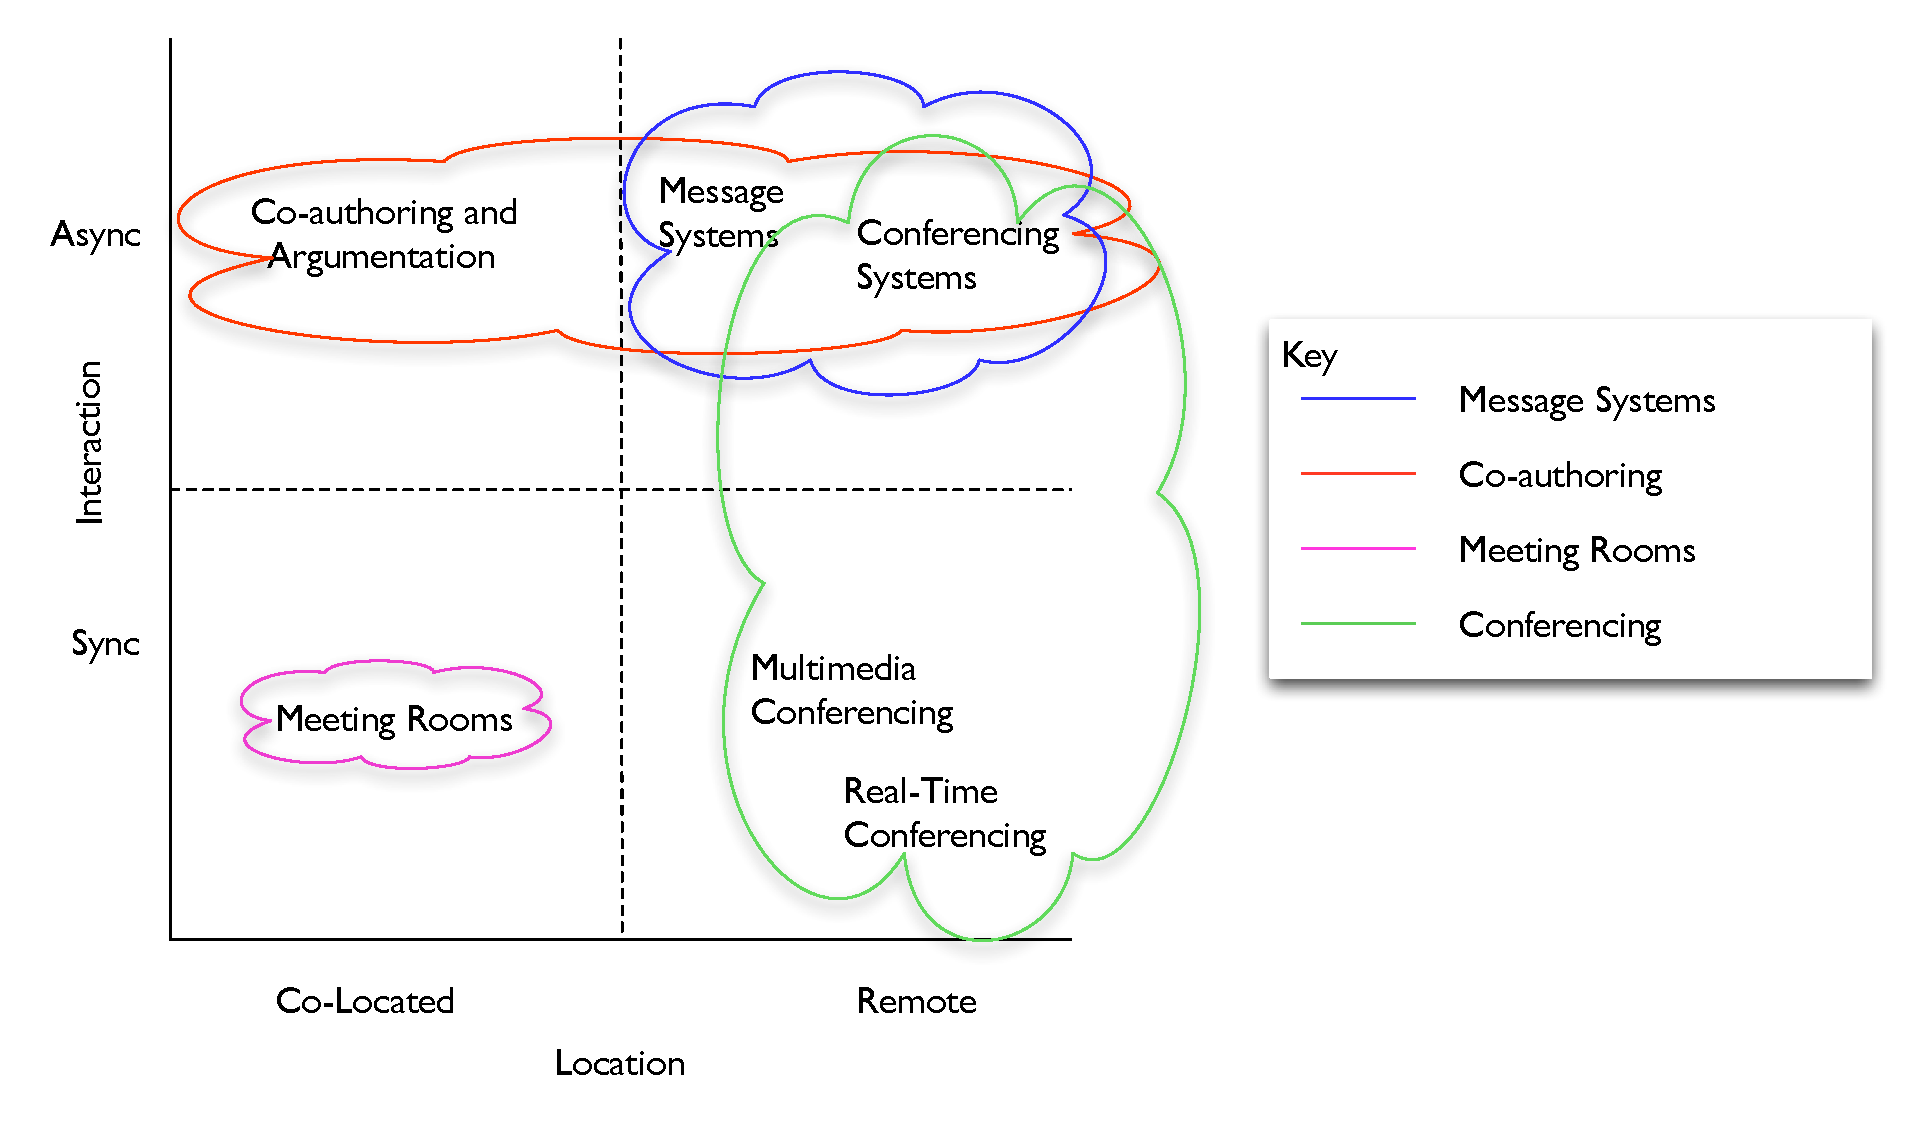
\includegraphics[width=140mm]{CSCWClass.eps}
  \label{CLASS_CSCW}
\end{figure}

\subsection{Message Systems}

\subsection{Conferencing systems}

\subsection{Meeting Rooms Systems}

\subsection{Co-authoring and Argumentation Systems}

\section{Biobike}

% This section can contain the introduction and objectives of biobike
% and where biobike fits in with the rest of the collaborative systems.
